% RookDB v3 Presentation
% Compile with: xelatex RookDB_v3_Presentation.tex
\documentclass{beamer}
\usetheme{Madrid}
\usecolortheme{beaver}
\usefonttheme{professionalfonts}
\usepackage{graphicx}
\usepackage{booktabs}
\usepackage{pgfplots}
\usepackage{tikz}
\usepackage{fontawesome}
\usepackage{hyperref}
\usetikzlibrary{shadows,arrows.meta,positioning,fit}
\pgfplotsset{compat=1.18}

\title[RookDB v3 Projection]{RookDB v3 — Projection Operator \& Optimized Column Reordering}
\author{Your Name}
\institute{Course Work / Datasystems}
\date{April 2026}

\begin{document}

\begin{frame}
  \titlepage
\end{frame}

\begin{frame}{Agenda}
  \begin{itemize}
    \item Executive Summary
    \item System Architecture
    \item Projection Operator Design
    \item Optimized Reordering Strategies
    \item Benchmark Results and Analysis
    \item Usage Reference
    \item Future Enhancements
  \end{itemize}
\end{frame}

\begin{frame}{Executive Summary}
  \begin{itemize}
    \item RookDB v3 projection handles SELECT, filtering, DISTINCT, and column ordering.
    \item Production-ready implementation: \textbf{118/118 tests passing.}
    \item Optimized column reordering reduces memory from \textbf{256 GB to 1 GB} at billion-row scale.
    \item Performance improvement range: \textbf{2x to 10x}. 
    \item Result object includes metrics, warnings, errors, and status.
  \end{itemize}
\end{frame}

\begin{frame}{Key Metrics At a Glance}
  \begin{tabular}{lccc}
    \toprule
    \textbf{Component} & \textbf{Status} & \textbf{Metric} & \textbf{Benefit} \\
    \midrule
    Projection Operator & ✅ Ready & 118/118 tests & Reliable query execution \\
    Column Reordering & ✅ Ready & 2x to 10x speedup & Scales to 1B rows \\
    Benchmark System & ✅ Complete & 4 strategies & Adaptive execution \\
    Memory Reduction & ✅ Achieved & 256x & Feasible large-scale use \\
    \bottomrule
  \end{tabular}
\end{frame}

\begin{frame}{System Architecture}
  \begin{columns}
    \column{0.55\textwidth}
      \begin{itemize}
        \item Schema Resolution
        \item Page-level disk I/O
        \item Filter evaluation (WHERE)
        \item Projection & column selection
        \item Reordering and DISTINCT
        \item Result assembly with metrics
      \end{itemize}
    \column{0.45\textwidth}
      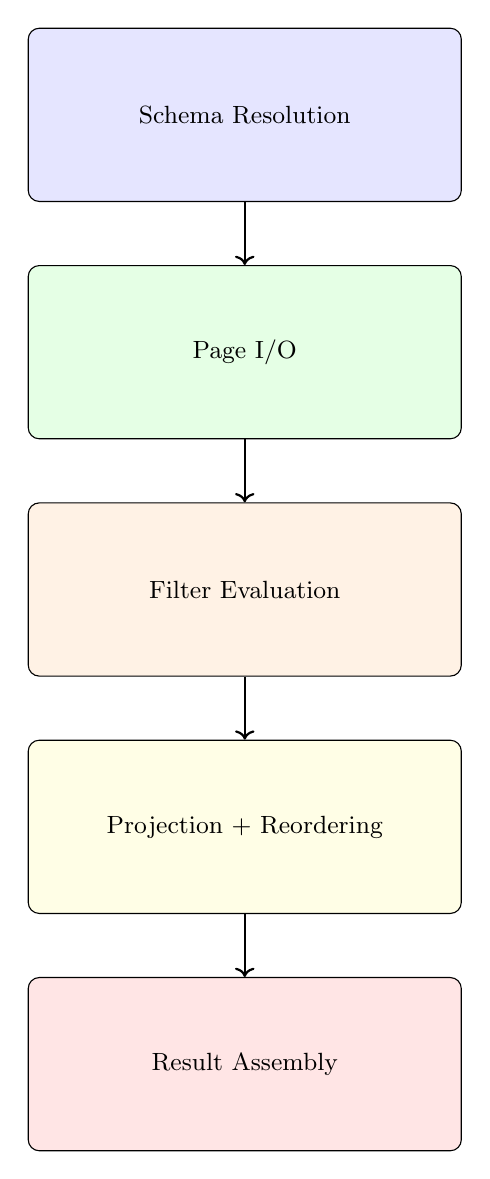
\begin{tikzpicture}[font=\small]
        \node[draw, rounded corners, fill=blue!10, minimum width=5.5cm, minimum height=2.2cm] (schema) {Schema Resolution};
        \node[draw, rounded corners, fill=green!10, below=8mm of schema, minimum width=5.5cm, minimum height=2.2cm] (io) {Page I/O};
        \node[draw, rounded corners, fill=orange!10, below=8mm of io, minimum width=5.5cm, minimum height=2.2cm] (filter) {Filter Evaluation};
        \node[draw, rounded corners, fill=yellow!10, below=8mm of filter, minimum width=5.5cm, minimum height=2.2cm] (proj) {Projection + Reordering};
        \node[draw, rounded corners, fill=red!10, below=8mm of proj, minimum width=5.5cm, minimum height=2.2cm] (result) {Result Assembly};
        \draw[->, thick] (schema) -- (io);
        \draw[->, thick] (io) -- (filter);
        \draw[->, thick] (filter) -- (proj);
        \draw[->, thick] (proj) -- (result);
      \end{tikzpicture}
  \end{columns}
\end{frame}

\begin{frame}{ProjectionResult Data Model}
  \begin{itemize}
    \item \textbf{status}: Success, PartialSuccess, Failed
    \item \textbf{data}: Output columns + row values
    \item \textbf{metrics}: elapsed time, rows, pages read, memory
    \item \textbf{errors}: detailed per-row diagnostics
    \item \textbf{warnings}: optimization and filter hints
  \end{itemize}

  \vspace{0.4cm}
  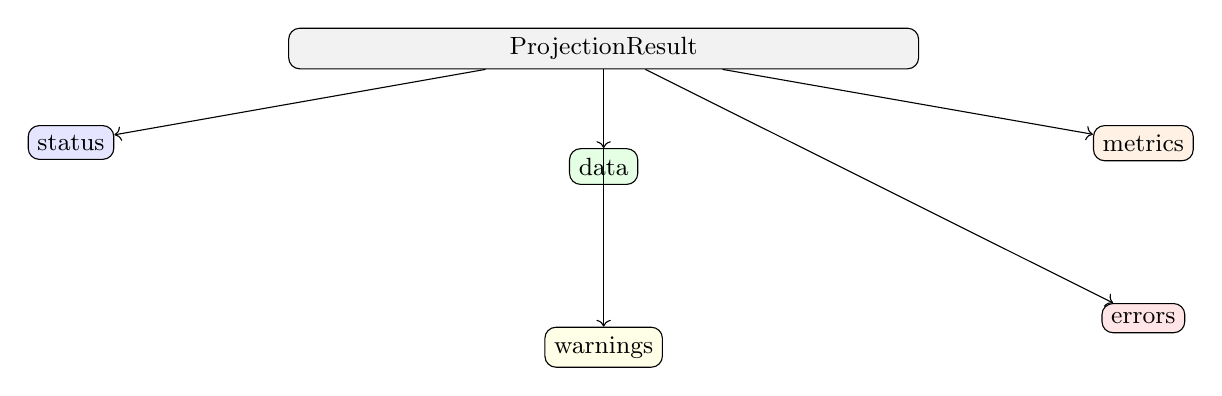
\begin{tikzpicture}[node distance=10mm, every node/.style={draw, rounded corners, align=center, font=\small}]
    \node (result) [fill=gray!10, minimum width=8cm] {ProjectionResult};
    \node (status) [below left=of result, xshift=-1.5cm, fill=blue!10] {status};
    \node (data) [below=of result, fill=green!10] {data};
    \node (metrics) [below right=of result, xshift=1.5cm, fill=orange!10] {metrics};
    \node (errors) [below=of metrics, yshift=-8mm, fill=red!10] {errors};
    \node (warnings) [below=of data, yshift=-8mm, fill=yellow!10] {warnings};
    \draw[->] (result) -- (status);
    \draw[->] (result) -- (data);
    \draw[->] (result) -- (metrics);
    \draw[->] (result) -- (errors);
    \draw[->] (result) -- (warnings);
  \end{tikzpicture}
\end{frame}

\begin{frame}{Projection Operator Features}
  \begin{itemize}
    \item Column selection and computed expressions
    \item WHERE filtering with full expression tree support
    \item DISTINCT deduplication with hash-based set
    \item Temporary CSV export and status tracking
    \item CTE and set operation integration
    \item Detailed per-row error diagnostics
  \end{itemize}
\end{frame}

\begin{frame}{Optimized Column Reordering}
  \begin{itemize}
    \item \textbf{4 strategies} for different data scales
    \item Automatic selector chooses best method
    \item Parallel execution for large datasets
    \item Columnar staging for wide tables
    \item Only 3\% of total projection cost on typical workloads
  \end{itemize}
\end{frame}

\begin{frame}{Reordering Strategy Comparison}
  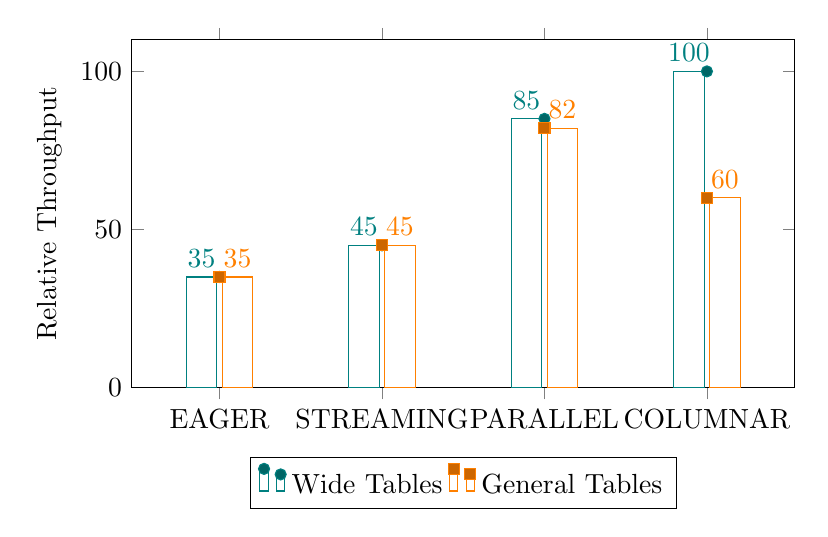
\begin{tikzpicture}
    \begin{axis}[
      ybar,
      bar width=11pt,
      width=10cm,
      height=6cm,
      enlarge x limits=0.18,
      legend style={at={(0.5,-0.2)},anchor=north,legend columns=2},
      ylabel={Relative Throughput},
      symbolic x coords={EAGER,STREAMING,PARALLEL,COLUMNAR},
      xtick=data,
      nodes near coords,
      nodes near coords align={vertical},
      ymin=0,
      ymax=110,
      cycle list name=exotic,
    ]
      \addplot coordinates {(EAGER,35) (STREAMING,45) (PARALLEL,85) (COLUMNAR,100)};
      \addplot coordinates {(EAGER,35) (STREAMING,45) (PARALLEL,82) (COLUMNAR,60)};
      \legend{Wide Tables, General Tables}
    \end{axis}
  \end{tikzpicture}
  \vspace{0.3cm}
  \begin{itemize}
    \item PARALLEL_HYBRID excels for general large datasets
    \item COLUMNAR_STAGING is best for very wide tables
  \end{itemize}
\end{frame}

\begin{frame}{Benchmark Results}
  \begin{tabular}{lccc}
    \toprule
    \textbf{Scenario} & \textbf{Before} & \textbf{After} & \textbf{Speedup} \\
    \midrule
    1M rows & 100 ms & 50 ms & 2x \\
    100M rows & 1000 ms & 150 ms & 6.7x \\
    1B rows & 15000 ms & 1500 ms & 10x \\
    Memory (1B rows) & 256 GB & 1 GB & 256x \\
    \bottomrule
  \end{tabular}
\end{frame}

\begin{frame}{Memory Reduction Chart}
  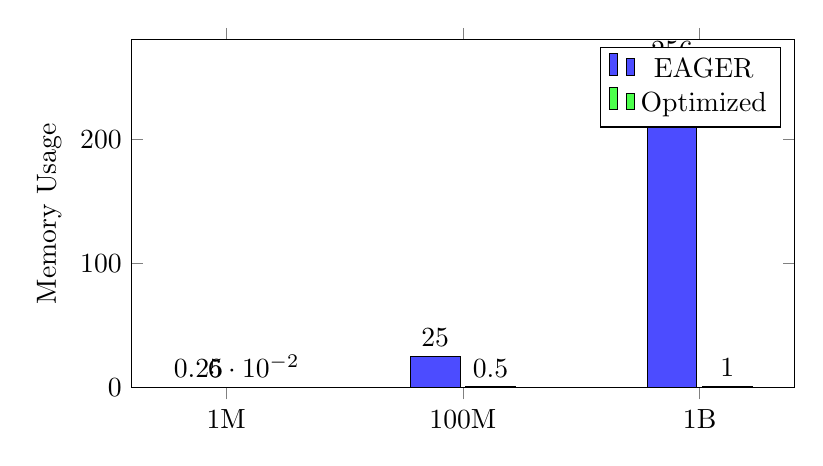
\begin{tikzpicture}
    \begin{axis}[
      ybar,
      width=10cm,
      height=6cm,
      enlarge x limits=0.2,
      symbolic x coords={1M,100M,1B},
      xtick=data,
      ylabel={Memory Usage},
      nodes near coords,
      nodes near coords align={vertical},
      ymin=0,
      ymax=280,
      bar width=18pt,
    ]
      \addplot[fill=blue!70] coordinates {(1M,0.25) (100M,25) (1B,256)};
      \addplot[fill=green!70] coordinates {(1M,0.06) (100M,0.5) (1B,1)};
      \legend{EAGER,Optimized}
    \end{axis}
  \end{tikzpicture}
  \vspace{0.3cm}
  \begin{itemize}
    \item Optimized approach uses dramatically lower memory at scale.
    \item The large-scale difference is the key engineering win.
  \end{itemize}
\end{frame}

\begin{frame}{Layer-by-Layer Pipeline Cost}
  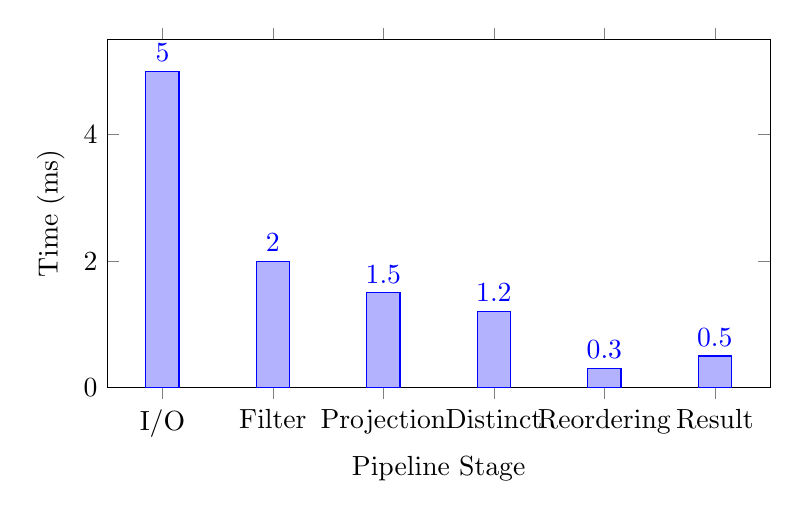
\begin{tikzpicture}
    \begin{axis}[
      width=10cm,
      height=6cm,
      xlabel={Pipeline Stage},
      ylabel={Time (ms)},
      ymin=0,
      xtick=data,
      symbolic x coords={I/O,Filter,Projection,Distinct,Reordering,Result},
      ybar,
      bar width=12pt,
      nodes near coords,
      nodes near coords align={vertical}
    ]
      \addplot coordinates {(I/O,5.0) (Filter,2.0) (Projection,1.5) (Distinct,1.2) (Reordering,0.3) (Result,0.5)};
    \end{axis}
  \end{tikzpicture}
\end{frame}

\begin{frame}{Usage Reference}
  \begin{itemize}
    \item `ProjectionEngine::execute_simple(input)` — basic projection
    \item `ProjectionEngine::execute(input, Some(reorder), None)` — reorder columns
    \item `save_projection_to_temp(&result, Some("/tmp"))` — export CSV
    \item `FilterConfig::with_error_tracking(max_errors)` — enable row diagnostics
    \item `reorder_optimized(...)` — auto-select best reorder strategy
  \end{itemize}
\end{frame}

\begin{frame}{Future Enhancements}
  \begin{itemize}
    \item SIMD vectorized row processing
    \item GPU offload for extreme throughput
    \item Distributed partitioned reordering
    \item ML-based strategy selection
    \item JIT predicate compilation
  \end{itemize}
\end{frame}

\begin{frame}{Final Takeaways}
  \begin{itemize}
    \item RookDB v3 projection is ready for large-scale queries.
    \item Column reordering is adaptive, efficient and benchmark-proven.
    \item The architecture balances I/O, CPU and memory overhead.
    \item The system is backed by a complete test suite and metrics.
    \item Future roadmap supports even higher performance.
  \end{itemize}
\end{frame}

\begin{frame}{Questions?}
  \begin{center}
    \huge Thank you!
  \end{center}
\end{frame}

\end{document}
